
\section{Elektrostatik}
\label{chap:Style}


Elektrisch geladene Teilchen, welche sich in der Nähe eines anderen, geladenen Teilchen befinden, verspüren eine Kraftwirkung, die Abhängig der eigenen Ladung ist. \\
Um diese Kraftwirkung zu beschreiben, wurde der Begriff des \textbf{Elektrischen Feldes} eingeführt.

\definition{Elektrisches Feld}
\beginip
Das elektrische Feld, beschreibt die Kraftwirkung auf geladene Teilchen im Raum. \\
Es ordnet jedem Punkt im Raum einen Vektor $\vec{E}$ zu, der in die Richtung der Kraftwirkung zeigt.
Für die Kraftwirkung auf ein Teilchen mit der Ladung Q und dem Ortsvektor $\vec{r}$ gilt: \\
\formulaBegin
$\vec{F} = Q \cdot \vec{E}(\vec{r})$
\formulaEnd
\iend

\vspace
\textbf{Einige wichtige Felder}
\bsp{Beispiel}{E-Feld einer Punktladung}
\beginbsp
Das elektrische Feld einer Punktladung Q ist gegeben als:
\formulaBegin
$\displaystyle \vec{E} = \frac{1}{4 \pi \epsilon} \cdot \frac{Q}{r^2}\cdot \vec{e}_r$
\formulaEnd
\begin{center}
	\ibox{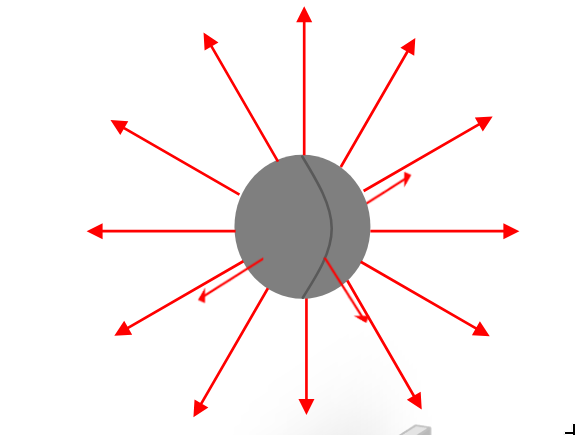
\includegraphics[scale=0.2]{img/e-feld-pkt.png}}
\end{center}
\iend




\bsp{Beispiel}{E-Feld einer Platte}
\beginbsp
Das elektrische Feld einer Platte mit Ladung Q ist gegeben als:
\formulaBegin
$\displaystyle \vec{E} = \begin{cases}
\frac{Q}{2\cdot A \varepsilon} \cdot \vec{e}_n & , y > y_0 \\
\frac{-Q}{2\cdot A \varepsilon} \cdot \vec{e}_n & , y \leq y_0 \\

\end{cases}
$
\formulaEnd
\begin{center}
	\ibox{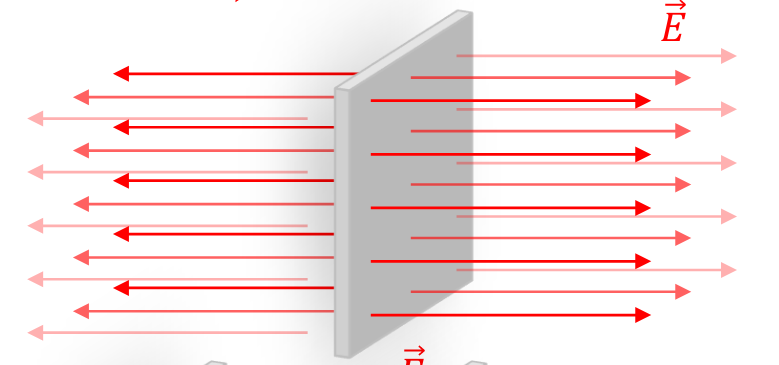
\includegraphics[scale=0.2]{img/e-feld-platte.png}}
\end{center}
\iend



\bsp{Beispiel}{E-Feld eines Kondensators}
\beginbsp
Das elektrische Feld in einem Kondensator mit der Ladung Q oder Spannung U ist gegeben als:
\formulaBegin
$\displaystyle \vec{E} = \frac{Q}{A\varepsilon} \cdot \vec{e}_d = \frac{U}{d	} \vec{e}_d$
\formulaEnd
\begin{center}
	\ibox{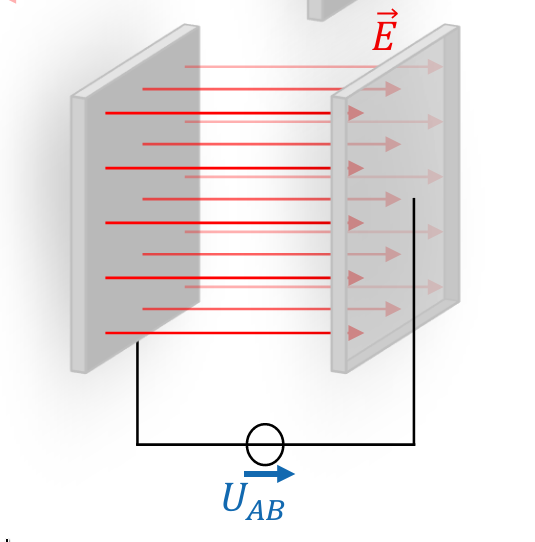
\includegraphics[scale=0.2]{img/e-feld-kond.png}}
\end{center}
\iend



\subsection{(Ladungs)-Dichte}
In der Physik sind wir häufig nicht nur daran interessiert, wieviele Ladungsträger sich in einem Volumen befinden, sondern wir möchten gerne Informationen darüber haben, wie sie geometrisch angeordnet sind. (= Verteilen sich alle Ladungsträger auf der Oberfläche, sind alle im Mittelpunkt zentriert etc). \\
Dazu werden \textbf{Dichtefunktionen} verwendet.

\definition{Linienladungsdichte $\lambda(x)$}
\beginip
Eine \textbf{Linienladungsdichte} gibt an, wie sich Ladungen entlang einer Linie anordnen. \\
Sind die Ladungsträger \textbf{gleichmässig} auf einer Linie verteilt, so ist die Dichte einfach eine Konstante mit Einheit $\frac{C}{m}$. \\
Möchten wir die Gesamtladung auf Basis einer Dichte berechnen, so müssen wir die Dichte Integrieren: \\
\formulaBegin
	$\displaystyle Q_{AB} = \int_A^B \lambda (x) \cdot dx$
\formulaEnd
\iend

\bsptask{Beispiel}{Linienladungsdichte}
\beginbsp
	Eine Gesamtladung von $Q=10C$ verteilt sich gleichmässig auf einer Gerade der Länge $l = 2m$. \\
	\begin{itemize}
		\item 1) Geben Sie die Linienladungsdichte $\lambda(x)$ im Bereich $ 0 < x <l$ an.
		\item 2) Geben Sie die Gesamtladung im eingeschlossenem Bereich $ 0 < x < l/3$ an.
	\end{itemize}
\iend

\newpage
\bsp{Lösung}{}
\beginbsp
\begin{itemize}
	\item 1) Da sich die Ladungen gleichmässig verteilen, ist die Ladungsdichte unabhängig vom Ort x
	\begin{center}
		$\lambda(x) = \lambda = \frac{C}{l} = 5 \frac{C}{m}$
	\end{center}
	\item 2) Die eingeschlossene Ladung berechnet sich Grundsätzlich mittels integration:
	\begin{center}
		$\displaystyle Q = \int_0^{l/3} \lambda(x) \cdot dx = \int_0^{l/3} 5 \frac{C}{m} \cdot dx = 5 \frac{C}{m} \cdot \frac{l}{3} = \frac{10}{3} C$
	\end{center}
\end{itemize}
\iend









\definition{Flächenladungsdichte $\sigma(x,y)$}
\beginip
Eine \textbf{Flächenladungsdichte} gibt an, wie sich Ladungen auf einer Fläche anordnen. \\
Sind die Ladungsträger \textbf{gleichmässig} auf der Fläche verteilt, so ist die Dichte einfach eine Konstante mit Einheit $\frac{C}{m^2}$. \\
Möchten wir die Gesamtladung auf Basis einer Dichte berechnen, so müssen wir die Dichte integrieren: \\
\formulaBegin
	$\displaystyle Q_{A} = \iint_A \sigma (x,y) \cdot dA$
\formulaEnd
Ist die Dichte konstant folgt:
\formulaBegin
	$\displaystyle Q_{A} = \sigma \cdot A$
\formulaEnd
\iend







\bsptask{Beispiel}{Flächenladungsdichte}
\beginbsp
	Eine Gesamtladung von $Q$ verteilt sich gleichmässig auf der Oberfläche einer Kugel mit Radius R. \\
	Wie Gross ist die Flächenladungsdiche $\sigma$ auf der Kugeloberfläche?
\iend


\bsp{Lösung}{}
\beginbsp
	Da sich die Ladungen gleichmässig verteilen, gilt für die Ladungsdichte:
	\begin{center}
		$\displaystyle \sigma = \frac{Q}{A} = \frac{Q}{4\pi R^2}$
	\end{center}
\iend






\newpage

\definition{Volumenladungsdichte $\rho(x,y,z)$}
\beginip
Eine \textbf{Volumenladungsdichte} gibt an, wie sich Ladungen in einem Volumen anordnen. \\
Sind die Ladungsträger \textbf{gleichmässig} im Volumen verteilt, so ist die Dichte einfach eine Konstante mit Einheit $\frac{C}{m^3}$. \\
Möchten wir die Gesamtladung auf Basis einer Dichte berechnen, so müssen wir die Dichte Integrieren: \\
\formulaBegin
	$\displaystyle Q_{V} = \iiint_V \rho (x,y,z) \cdot dV$
\formulaEnd
Ist die Dichte konstant folgt:
\formulaBegin
	$\displaystyle Q_{V} = \rho \cdot V$
\formulaEnd
\iend




\bsptask{Beispiel}{Volumenladungsdichte}
\beginbsp
Eine Hohlkugel mit Innenradius $R_1$ und Aussenradius $R_2$ sei im Bereich $ R_1 \leq r \leq R_2$ gleichmässig mit der Ladung $Q$ gefüllt. \\
Gesucht ist die Volumenladungsdichte $\rho(r,\theta,\varphi)$ in Kugelkoordinaten, welche die Ladungsdichte im gesamten Raum beschreibt.
\iend


\bsp{Lösung}{}
\beginbsp
Da sich die Ladungen nur in einem gewissen Teil des Raumes befinden, müssen wir eine Fallunterscheidung durchfüren:
\begin{enumerate}
	\item $\mathbf{r < R_1}$ \\
	Hier befindet sich keine Ladung, somit ist auch die Volumenladungsdichte gleich 0
		\item $\mathbf{R_1 \leq r \leq R_2}$ \\
		Hier ist die Ladung gleichmässig auf dem Volumen $V = 4\cdot \pi (R_2^3 - R_1^3)$ verteilt, somit beträgt die Volumenladungsdichte:
		\begin{center}
			$\displaystyle \rho = \frac{Q}{V} = \frac{Q}{4 \cdot \pi (R_2^3 - R_1^3) }$
		\end{center}
		\item $\mathbf{r > R_3}$ \\
		Hier befindet sich keine Ladung, somit ist auch die Volumenladungsdichte gleich 0
\end{enumerate}

Somit gilt für die ortsabhängige Volumenladungsdichte:
\begin{center}
	$\displaystyle	\rho(r,\theta,\varphi) =
		\begin{cases}
			0                                       & r < R_1 \\
		 \frac{Q}{4 \cdot \pi (R_2^3 - R_1^3)} & R_1 \leq r \leq R_2\\
				0                                       & r > R_2 \\
		\end{cases}$
\end{center}

\iend


\newpage

\subsection{Elektrische Flussdichte}
Quelle des elektrischen Feldes sind geladene Teilchen. Jedoch hängt das elektrische Feld davon ab, in was für einem Material wir uns befinden. \\
Das elektrische Feld in einem Metall ist zum Beispiel kleiner, als das elektrische Feld im Vakuum. \\
Grund dafür ist die \textbf{elektrische Influenz}, welche das Ursprüngliche Feld abschwächt \\
Um gewisse Rechnungen zu vereinfachen, definieren wir ein neues Feld.

\important{Definition}{Die elektrische Flussdichte}
\beginip
Die elektrische Flussdichte $\vec{D}$ beschreibt das Feld, welches existieren würde, falls kein Material vorhanden wäre. \\
Quelle der elektrischen Flussdichte ist die elektrische Ladung Q.
\iend

Da die elektrische Flussdichte  $\vec{D}$ unabhängig vom Material ist und aussschliesslich von den Ladungsträger abhängig ist,
gibt es eine Formel, die die beiden Grössen in Verbindung bringt:

\gl{Gleichung}{Quellgleichung des elektrischen Flusses}

\begingl
\begin{center}
	\formulaBegin
	$\Psi := \oiint \vec{D}\cdot d\vec{A} = \iint_V \rho dV = Q_{eff}$
	\formulaEnd

	Falls Feld senkrecht auf Fläche und Konstant \\
	\fspace

	\formulaBegin
	$D = |\frac{Q_{eff}}{A_{eff}}|$
	\formulaEnd

\end{center}
\textbf{Variabeln}: \\
$\Psi = $ Elektrischer Fluss $ [\Psi] = A \cdot s $ \\
$D = $ Elektrische Flussdichte $ [D] = \frac{As}{m^2}$ \\
$ Q_{eff} = $ Von der Fläche eingeschlossene Ladung $[Q] = A\cdot s$ \\
$ A_{eff} = $ Fläche, durch die das D-Feld durchfliesst$ [A] = m^2$ \\

\iend

\bsptask{Beispiel}{Berechnung des D-Feldes einer Kugel}
\beginbsp
Eine Kugel sei mit der Ladung $20 C$ gefüllt. Die Kugel habe den Radius $R = 2cm$ und alle Ladungsträger verteilen sich auf der Kugeloberfläche. \\
Berechne das $\vec{D}$-Feld der Kugel.
\iend


\newpage


\important{Lösung}{}
\beginbsp
Um das D-Feld der Kugel anzugeben, müssen wir zuerst ein passendes Koordinatesystem wählen. \\
Da wir mit einer Kugel rechnen, muss das Feld Punktsymmetrisch sein und einzig der Abstand zum Kugelmittelpunkt bestimmt, wie gross das D-Feld ist. \\
Aufgrund dieser Überlegung, werden wir \textbf{Kugelkoordinaten} verwenden. (Hätten wir etwas, das Symmetrisch zur Z-Achse ist, so würden wir Zylinderkoord. verwenden etc.). \\
Um die Gleichung für den Elektrischen Fluss anwenden zu können, müssen wir eine Hüllfläche finden,   \textbf{auf der das D-Feld Konstant ist}. \\
Da die Anordnung eine Kugel ist, verwenden wir als Hüllfläche eine Kugel mit Radius r. \\
Nun können wir die Quellgleichung verwenden:
\begin{center}
	$ \oiint_A \vec{D}\cdot d\vec{A} = Q_{eff} \rightarrow D \cdot  4\pi r^2  = Q_{eff} $
\end{center}
Der Betrag des D-Feldes entspricht also gerade der von der Hullfläche eingeschlossenen Ladung geteilt durch die Fläche. \\
Für den Fall, dass wir die Hüllfläche grösser als die Kugel wählen, schliessen wir alle Ladungen ein: \\
$\mathbf{r \beq R}$ \\
\begin{center}
	$Q_{eff} = 20C$ \\
	$D = \frac{20C}{4\pi r^2}$ \\
	$\vec{D} = D \cdot \vec{e}_r$
\end{center}

Falls unsere Hüllfläche im inneren der Kugel ist, so schliessen wir keine Ladung ein: \\
$\mathbf{r < R}$ \\
\begin{center}
	$Q_eff = 0C$ \\
	$\vec{D} = 0$
\end{center}

Somit gilt für das D-Feld einer Kugel mit Ladungen auf der Oberfläche: \\
\begin{center}

	$ \displaystyle
	\vec{D}(r) =
	\begin{cases}
		0                                       & r < R \\
		\frac{20 C}{4 \pi r^2} \cdot  \vec{e}_r & r \beq R \\
	\end{cases}$

\end{center}
\iend



\newpage

Da die elektrische Flussdichte nur von den Ladungsträgern abhängig ist, lässt sie sich realtiv einfach berechnen und bildet meist den Grundstein für
das Berechnen von E-Feldern usw. \\
\texttt{"}Fliesst\texttt{"} eine elektrische Flussdichte durch ein Material mit Ladungsträgern, so wird diese abgeschwächt, da sich im inneren des Materiales ein
elektrisches Feld entgegen dem von Aussen angelegtem Feld ausbildet. \\
\begin{center}
	\ibox{
		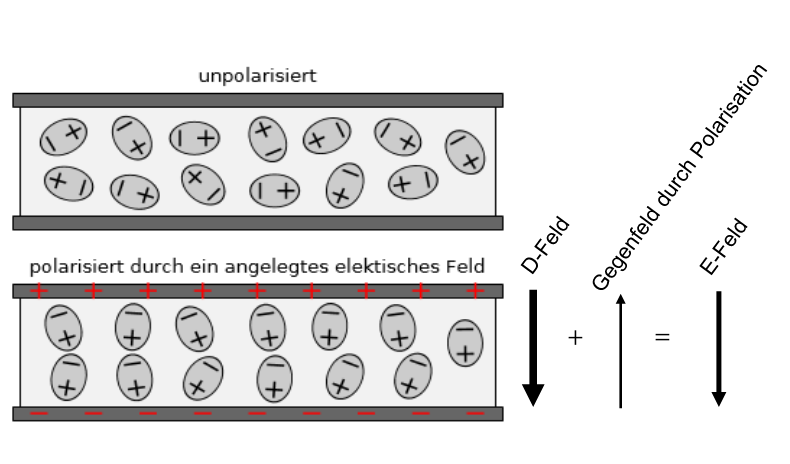
\includegraphics[scale=0.4]{img/d-e-feld.png}}
\end{center}

\gl{Gleichung}{Zusammenhang E-Feld und D-Feld}
\begingl
\begin{center}
	\formulaBegin
	$ \vec{E} = \frac{1}{\varepsilon_0 \cdot \varepsilon_r} \cdot \vec{D}$
	\formulaEnd
\end{center}
\textbf{Variabeln}: \\
$D = $ Elektrische Flussdichte $ [D] = \frac{As}{m^2}$ \\
$ E = $ Elektrisches Feld $[E] = \frac{V}{m}$ \\
$ \varepsilon_0 = $ Dielektrizitätskonstante $ [\varepsilon_0] = \frac{C}{V\cdot m}$ \\
$ \varepsilon_r = $ rel. Permitivität. Unterschiedlich im Material $ [\varepsilon_r] = [ ]$ \\

\iend


\newpage


\definition{Verhalten von Feldgrössen bei Materialübergängen}
\beginip
Trifft eine Eelektrische Flussdichte durch eine geladene Fläche, so verändert sich die Normalkomponente des D-Feldes. \\
Die Tangentialkomponente des Feldes bleibt jedoch konstant. \\
 \begin{center}
	 \ibox{
	 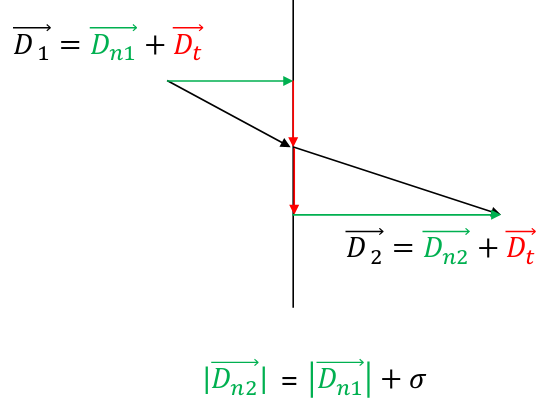
\includegraphics[scale=1.5]{img/dfield.png}}
\end{center}
\formulaBegin
$\vec{D}_1 = \vec{D}_{1t} + \vec{D}_{1n} \Rightarrow \vec{D}_2 = \vec{D}_{1t} + (1 + \sigma) \cdot \vec{D}_{1n}$
\formulaEnd
\iend

\definition{Spannung}

\beginip
Wir definieren die Spannung zwischen zwei Punkten als das Wegintegral über das elektrische Feld: \\
\formulaBegin
$ U_{AB} :=  \int_A^B \vec{E} \cdot d\vec{s} $
\formulaEnd
{[U]} = Volt {[V]}
\iend

\paragraph{Bemerkung zur Spannung}

\begin{itemize}

	\item	Da die Beziehung $\vec{F} =  q \cdot \vec{E} $ gilt und die Arbeit als $ W_{AB} = \int_A^B \vec{F} \cdot d\vec{s}$ definiert ist, können wir die Spannung zwischen zwei Punkten als \textbf{Maß der benötigten Arbeit} um ein Ladungsträger von A nach B zu bringen betrachten.  \\
	\item Die Spannung ist unabhängig des Weges.  $U_{AC} = U_{AB} + U_{BC}$
	      \\ $\Rightarrow$ Start- und Endwert sind ausreichend. \\
	\item Die Spannung über einen Weg zurück zum Anfangsort entspricht \textbf{0V}: $U_{AB} + U_{BA} = 0$ \\
	\item Ist die Spannung auf dem gesamten Weg konstant und parallel zum Weg, vereinfacht sich das Integral zu einer Multiplikation: \\
	      \begin{center}
	      	$ U_{AB} = \int_{A}^{B} \vec{E}\cdot d\vec{s} = l_{AB} \cdot E$
	      \end{center}
\end{itemize}


\newpage
\subsection{Vorgehen zur Feldberechnung}
\vorgehen{Vorgehen}{Feldberechnungen für eine gegebene Anordnung}
\beginvor
Zuerst: Besteht die Anordnung aus bekannten Teilobjekten (Kugeln mit verschiedenen Radien etc?) \\
$\rightarrow$ Wende \textbf{Superposition} an: Berechne das Feld jeder einzelnen Teilanordnung mithilfe des Vorgehens und summiere Resultate auf.
\\
\begin{itemize}

	\item [1. ] Versuche die Symmetrie der Anordnung herauszufinden und entscheide dich für ein Koordinatensystem: \\
	Punktsymmetrisch $\rightarrow$ Kugelkoordinaten \\
	Achsensymmetrisch $\rightarrow$ Zylinderkoordinaten \\
	Symmetrisch zu einer Ebene $\rightarrow$ Karthesischekoordinaten\\

	\item [2. a]Falls \textbf{Ladungsdichte oder Ladung} gegeben: \\
\end{itemize}
	\beginip
	\begin{itemize}

	\item [2. 1]  Suche Hüllfläche, auf der das Feld Konstant ist


	\item [2. 2] Verwende $\displaystyle \oiint_A \vec{D} \cdot d\vec{A} = Q \Rightarrow D = \frac{Q_{eff}}{A_{eff}}$ \\
	Je nach Hüllfläche muss hier eine Fallunterscheidung gemacht werden, da ggf. sich die eingeschlossene Ladung $Q_{eff}$ ändern könnte\\
	Falls das D-Feld senkrecht durch verschiedene Materialien fliesst, bleibt es überall Konstant.

	\item [2. 3] Aus Skizze, finde heraus, in welche Richtung das D-Feld zeigt und ergänze den Richtungsvektor:
	\begin{center}
		$\vec{D} = D \cdot \vec{e}_D$
	\end{center}

	\item [2. 4] Das resultierende E-Feld in en einzelnen Materialien mit $\varepsilon_{ri}$ ist gegben als:
	\begin{center}
			$\displaystyle \vec{E} = \frac{\vec{D}}{\varepsilon_0 \cdot \varepsilon_{ri}}$
	\end{center}
\end{itemize}
\iend
\begin{itemize}
	\item [2. b] Falls \textbf{Spannung} zwischen Punkten gegeben ist:\\

	\end{itemize}
	\beginip
	\begin{itemize}

	\item [2. 1]  Suche eine Weg vom Punkt A zum Punkt B, auf dem das Feld konstant ist. \\

	\item [2. 2] Verwende $\displaystyle U_{AB} = \int_A^B \vec{E}\cdot d\vec{s}$ \\
	$\displaystyle \rightarrow E = \frac{U_{AB}}{l_{AB}}$

	\item [2. 3] Aus Skizze, finde heraus, in welche Richtung das E-Feld zeigt und ergänze den Richtungsvektor:
	\begin{center}
		$\vec{E} = E \cdot \vec{e}_E$
	\end{center}
	\end{itemize}
	\iend
\iend


\newpage
\subsection{Kondensator}

Bringen wir 2 Platten mit verschiedenen Ladungsträger nah zu einander, so bildet sich ein elektrisches Feld zwischen den Platten. \\
Die Stärke des elektrischen Feldes ist abhängig der Plattenladung und der Flächen der Platten.

\fix
\fix
\fix
\definition{Kondensator}
\beginip
Ein Kondensator ist ein Bauelement, das in der Lage ist elektrische Ladung und somit Energie in Form von Feldlinien zu speichern. \\
Die charakteristische Kenngrösse des Kondensators ist die Kapazität \textbf{C}. \\
Die im Feld eines Kondensators gespeicherte Energie entspricht $\mathbf{W = \frac{1}{2} C \cdot U^2}$ \\
\iend



\fix
\fix
\fix
\definition{Kapazität}
\beginip
Die elektrische Kapazität C beschreibt die Fähigkeit eines Bauelementes, Ladung $Q$ bei einer gewissen Spannung $U$ zu speichern. \\
Als Proportionalitätsgrösse gibt sie an, wie gross die Spannung über einem Bauelement bei einer Ladung Q ist.
\formulaBegin
$C =\displaystyle \frac{Q}{U}$
\formulaEnd
In Abhängigkeit der Felder, lässt sich die Kapazität folgendermassen beschreiben:
\formulaBegin
$ C = \displaystyle \frac{\oiint_A \vec{D} \cdot d \vec{A} }{ \int_s \vec{E} \cdot d\vec{s}}$
\formulaEnd
Falls das Feld senkrecht auf der Hüllfläche steht und der Integrationsweg parallel zum E-Feld verläuft gilt:
\formulaBegin
$ C= \displaystyle \frac{D \cdot A_{eff} } {\int_A^B E \cdot ds} $
\formulaEnd
\iend


\gl{Gleichung}{Kapazität eines Plattenkondensators}
\begingl
Bei einem Plattenkondensator mit Fläche A und Abstand d, der mit einem Dielektrikum mit Konstante $\varepsilon$ gefüllt ist, gilt: \\
\formulaBegin
$ \displaystyle C = \varepsilon \cdot \frac{A}{ d}$
\formulaEnd

\textbf{Variabeln}: \\
$A = $ Fläche einer Platte $ [A] = m^2 $ \\
$d = $ Abstand der Platten $ [d] = m$ \\
$ \varepsilon = \varepsilon_0 \cdot \varepsilon_r $ Dielektrikum zw. den Platten $ [\varepsilon] = \frac{C}{V\cdot m}$ \\

\iend

\textbf{Begründung}
Da das E-Feld eines Plattenkondensators Konstant ist, gilt für die Kapazität:
\fix
\fix
\begin{center}
	$ C= \displaystyle \frac{D \cdot A_{eff} } {E \cdot d} $
\end{center}
\fix
\fix
Mit dem Zusammenhang $ D = \varepsilon \cdot E$ und der Erkenntniss, dass das Feld nur auf der einen Seite der Platte existiert folgt:
\fix \fix
\begin{center}
	$ C= \displaystyle \frac{E \cdot \varepsilon \cdot A_{eff} } {E  \cdot d}  = \doubleunderline{\displaystyle \varepsilon \frac{A} { d}}$
\end{center}



\definition{Serienschaltung von Kapazitäten}

\beginip
Werden mehrere Kapazitäten seriell miteinander verbunden, so addieren sich die Kehrwerte der Kapazität \\
\formulaBegin
$\displaystyle \frac{1}{C_{ges}} = \sum_{i=0}^n \frac{1}{C_i} \Bigg\rvert$
$\displaystyle C_{ges} = \frac{C_1 \cdot C_2}{C_1 + C_2} = (C_1 || C_2)$
\formulaEnd
\iend


\textbf{Begründung} \\
Die Definition der Kapazität ist genau gegensätzlich zu der des Widerstandes ($ R \propto \frac{l}{A}$ , $ C \propto \cdot \frac{A}{d} $)\\
Werden Kondensatoren in Serie geschaltet, so vergrößert sich der effektive Abstand der Platten, weshalb wir die Kehrwerte addieren müssen. \\



\definition{Parallelschaltung von Kapazitäten}

\beginip
Werden mehrere Kapazitäten parallel miteinander verbunden, so addieren sich die Kapazitäten \\
\formulaBegin
$\displaystyle C_{ges} = \sum_{i=0}^n C_i $
\formulaEnd
\iend

\definition{Ladungserhaltung in der Serienschaltung}
\beginip
Werden Kapazitäten in Serie geschaltet, besitzen alle dieselbe Ladung Q.
\begin{center}
	\fix
	\ibox{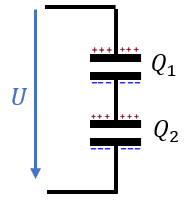
\includegraphics[scale=0.5]{img/kond1.png}} $\displaystyle \doubleunderline{Q_1 = Q_2 = Q}$
\end{center}
\iend

\textbf{Begründung} \\
Damit sich auf dem ersten Kondensator die Ladung $Q_1$ ansammeln kann, muss diese Ladung unterhalb des Kondensators angesammelt werden. Angenommen, beide Kondensatoren waren zu Beginn ungeladen,
so muss die Ladung, welche sich auf der unteren Platte des ersten Kondensators befindet, dieselbe Ladungsmenge auf der oberen Platte des unteren Kondensators hervorrufen. \\
\fix
\fix
\fix
\definition{Maschenregel bei Parallelschaltung}
\beginip
Die Maschenregel für Spannung gilt auch bei Kondensatoren
\begin{center}
	\fix
	\ibox{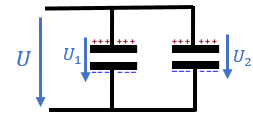
\includegraphics[scale=0.5]{img/kond2.png}}
	$\displaystyle \doubleunderline{U_1 = U_2 = U} $  und  $\displaystyle C_1 = \frac{Q_1}{U_1} \rightarrow \doubleunderline{Q_1 = C_1 \cdot U}$
\end{center}
\iend
